\secnumbersection{Definición del problema} 
\hlabel{sec:1}

Teniendo como contexto el creciente uso de programación en GPUs, es que nace el concepto de GPGPU (del ingles, General-Purpose computing on Graphics Processing Units) y es que se plantea el problema a tratar en esta memoria.
Este concepto consta de un cambio en el rol de las tarjetas gráficas, desde renderizar todo lo relacionado al despliegue gráfico de un computador, al uso de su gran cantidad de recursos de procesamiento en temas más generales.
Por esta razón, es que se han generado una cantidad considerable de plataformas de desarrollo las cuales permiten crear códigos apuntados a ejecutarse en GPUs que aprovechen las características de su arquitectura, sobre todo el uso de computación paralela \cite{gpuev}.

\begin{figure}[h]
    \centering
    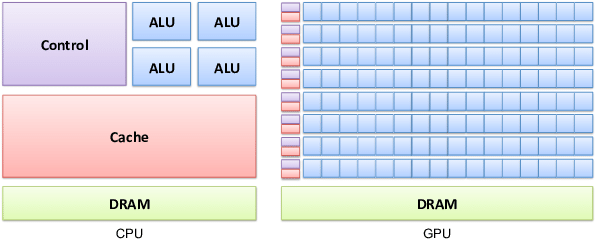
\includegraphics[scale=0.7]{Figures/arch.png}
    \caption{Arquitectura CPU versus GPU, fuente: \cite{arch}.}
    \label{fig:1}
\end{figure}

Las plataformas de desarrollo más actuales tienen como característica una compilación más enfocada en que la ejecución de los binarios esté optimizada a la arquitectura y los núcleos presentes en la GPU que se utilice y que no presente problemas en el paralelismo, como cumplir condiciones de carrera, consistencia en la escritura/lectura, etc.
Actualmente dentro de este tipo de entorno de software, destacan OpenCL, Halide, ROCm y CUDA, sin embargo este último ha tenido una popularidad mayor, al ser desarrollado y distribuido de forma \textit{open-source} por NVIDIA para ser utilizado únicamente por GPUs de la misma compañía.
Debido a esta restricción existente, es que se plantea el uso de ROCm \cite{rocm} para la implementación de esta memoria, ya que es desarrollado por AMD y se plantea como alternativa directa de CUDA y NVIDIA.

Además, dentro de las características favorables del uso de ROCm se encuentra el lenguaje de programación HIP (acrónimo en inglés de Heterogeneous-Computing Interface for Portability), el cual tiene la capacidad computacional de tanto ejecutar código de ROCm en tarjetas gráficas AMD como de traducir código a lenguaje CUDA y ejecutarlo en tarjetas gráficas NVIDIA, gracias a la herramienta Hipify.

\begin{figure}[h]
    \centering
    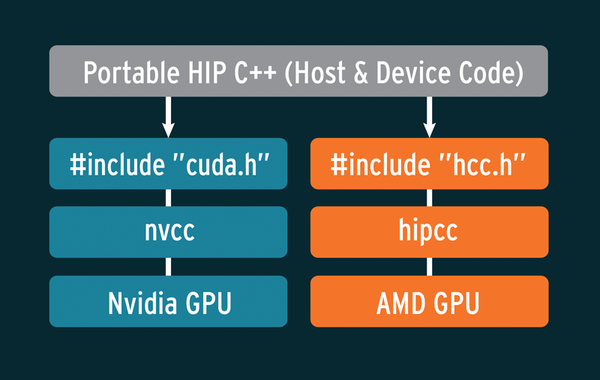
\includegraphics[height=.4\textwidth]{Figures/hipify.png}
    \caption{Diagrama de flujo desde HIP hasta el dispositivo utilizado.}
    \label{fig:2}
\end{figure}

Por otro lado, hasta la última versión lanzada de ROCm, esta tiene soporte para variadas librerías asociadas al uso de HCP, destacando como por ejemplo:

\begin{itemize}
    \item rocBLAS: Conjunto de rutinas asociadas a la ejecución de BLAS (del inglés, Basic Linear Algebra Subprograms), la cual especifica rutinas de bajo nivel sobre operaciones de algebra linear. Este conjunto de software comprende los 3 niveles de operaciones BLAS:
    \begin{itemize}
        \item Nivel 1, sobre operaciones vectoriales en matrices escalonadas, o del tipo 
        \begin{equation*}
            \mathbf{a}\leftarrow \alpha \mathbf{x} + \mathbf{y}
        \end{equation*}
        en donde $\mathbf{a},\mathbf{x},\mathbf{y} \in \mathbb{R}^{n}$ y $\alpha \in \mathbb{R}$.
        \item Nivel 2, sobre operaciones matriz-vector generalizadas (también conocidas como \textit{gemv}), o del tipo
        \begin{equation*}
            \mathbf{a} \leftarrow A\mathbf{x} + \beta \mathbf{y}
        \end{equation*}
        en donde $\mathbf{a},\mathbf{x},\mathbf{y} \in \mathbb{R}^n$, $A \in \mathbb{R}^{n\times n}$ y $\beta \in \mathbb{R}$.
        \item Nivel 3, sobre operaciones matriz-matriz generalizadas (también conocidas como \textit{gemm}), o del tipo
        \begin{equation*}
            A \leftarrow \alpha X\,Y + \beta Z
        \end{equation*}
        en donde $X,Y,Z \in \mathbb{R}^{n\times n}$ y $\alpha,\beta \in \mathbb{R}$.
    \end{itemize}
    \item PyTorch, TensorFlow, Caffe: Librerías asociadas a la construcción, entrenamiento y evaluación de redes neuronales. 
    Estas son útiles al momento de querer entrenar una red neuronal utilizando una gran cantidad de neuronas junto a un gran volumen de datos de entrenamiento, lo cual implicaría un alto costo computacional en caso de desarrollarse de forma secuencial.
    \item rocFFT: Librería de software para computar transformadas rápidas de fourier (del inglés, Fast Fourier Transform), escrita en HIP¨.
\end{itemize}

\begin{figure}[ht]
    \centering
    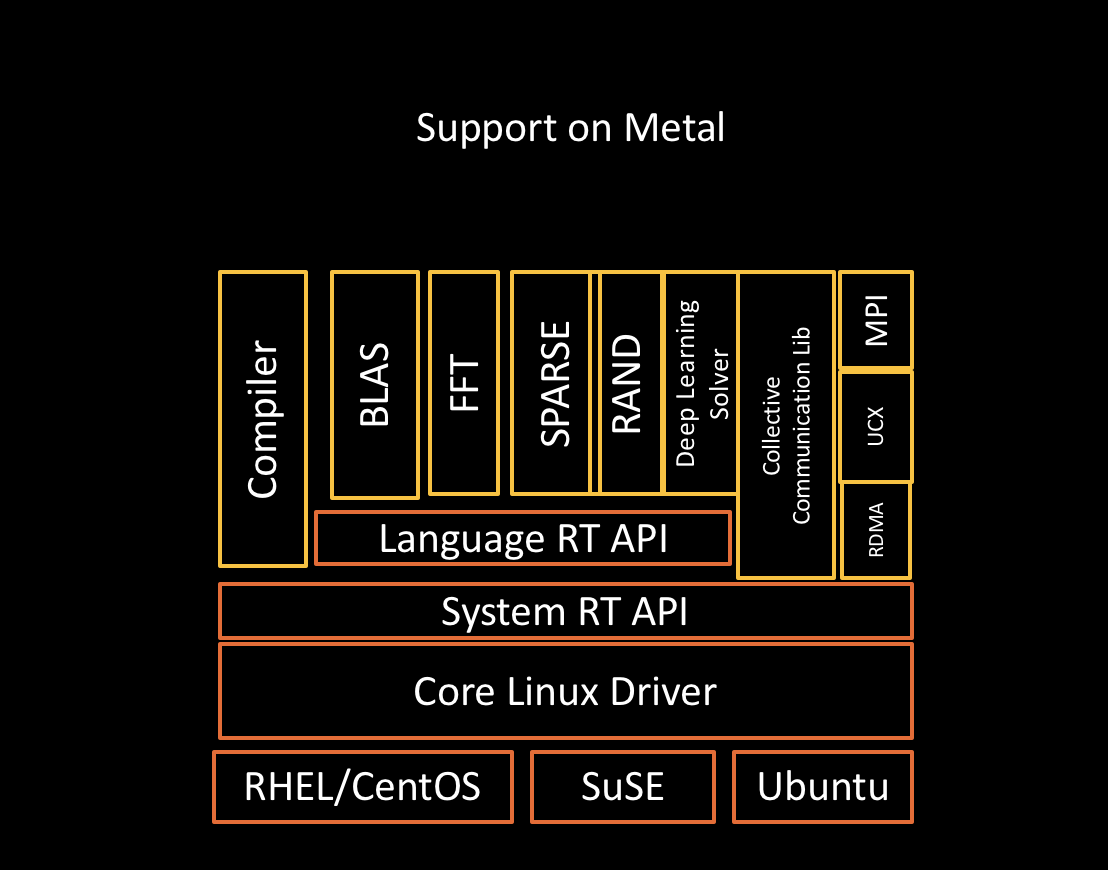
\includegraphics[height=.4\textwidth]{Figures/library.png}
    \caption{Soporte de librerías de ROCm}
    \label{fig:3}
\end{figure}

Respecto a la teoría que se utilizará para sostener las simulaciones a realizar, se seleccionó el método de Lattice Boltzman debido a su aceptación dentro del área de dinámica de fluidos y por el reciente aumento en su implementación sobre frameworks o software en general. 
Junto al método de Lattice Boltzmann base se considerarán condiciones de borde abiertas con tal de poder representar una continuidad de los fluidos.
Esto aumenta la utilidad de las simulaciones generadas, al asemejarlas aun más al comportamiento de fluidos en la vida real.
%asemejar los fluidos simulados a aquellos comportamientos en la vida real y por tanto la utilidad de las simulaciones generadas.
También, se espera poder plantear condiciones iniciales de diferentes simulaciones que permitan representar posibles tsunamis dentro de la costa Chilena (Figuras~\ref{fig:25}-\ref{fig:27}), esperando que sean un beneficio sobre la toma de decisiones al momento de la ocurrencia de uno después de la de un terremoto, pues como es de conocimiento publico, Chile es uno de los países más sísmicos del mundo junto con Japón~\cite{quake}.
Finalmente, uno de los legados principales de esta memoria será una implementación del método de Lattice Boltzmann en la plataforma ROCm, ya que, al ser esta un software sin un uso masificado, no presenta existencias de implementaciones de simulaciones de mecánica de fluidos en general.